\chapter{Méthodes numériques}
\label{chap-sim}

En 1949, Metropolis \cite{metropolis_monte_1949} découvre une méthode pour calculer via des simulations numériques de Monte Carlo, la moyenne d'observables statistiques. Si $Q$ est une quantité observable appartenant à un système statistique, comme l'énergie interne ou la densité moyenne de particules par site, alors la moyenne est calculée en pondérant la valeur de l'observable sur toutes les configurations $C$ du système par rapport au poids statistique de ces configurations. Si l'on considère le système en équilibre thermodynamique alors chaque configuration $C$ suit une distribution de Gibbs-Boltzmann, et la moyenne $<Q>$ est vaut
\begin{align}
    <Q> = \frac{\sum_{C} Q(C) \exp(-\beta E(C))}{\sum_{C} \exp(-\beta E(C))}
\end{align}
Pour un système SOS de taille $100\times100$ par exemple, petit par rapport à la limite thermodynamique comme discuté avec la figure \ref{fig-thermo-libre}, il existe $100^{100}$ configurations possibles, bien qu'une simulation numérique ne puisse explorer qu'environ $10^8$ configurations différentes en un temps CPU raisonnable.
Les modèles sur réseau se prêtent parfaitement aux simulations numériques de Monte Carlo, où le but est de calculer la valeur moyenne des observables telles que l'énergie interne ou la densité moyenne de particule par site. Toutes ces quantités peuvent être calculées directement pour le modèle SOS dans l'ensemble grand-canonique à l'aide des valeurs propres de la matrice de transfert, mais il est impossible d'utiliser une telle méthode dans l'ensemble canonique, comme expliqué dans le chapitre précédent.

Dans ce chapitre, nous commençons par expliquer le principe des simulations de Monte Carlo Metropolis, et comment choisir l'ensemble thermodyique de la simulation numérique. En plus d'étudier l'ensemble canonique, les simulations numériques offrent la possibilité d'étudier les régimes hors équilibre, dont nous justifierons la validité.
Nous finirons le chapitre par expliquer comment accélérer la vitesse de simulation grâce à la parallélisation, ainsi que d'autres astuces de programmation, en insistant sur les écueils techniques à éviter. 

Je remercie le Mésocentre de Calcul Intensif Aquitain (MCIA)\footnote{\url{https://redmine.mcia.fr/projects/mcia}} sur lequel j'ai effectué la très grande majorité de mes simulations numériques. 
L'intégralité du code produit pour cette thèse est accessible sur Github \footnote{\url{https://github.com/Bulbille/Curta}} sous la licence Creative Commons BY 3.0 \footnote{\url{https://creativecommons.org/licenses/by/3.0/fr/}}. Les simulations numériques ont été codées en C++, la parallélisation avec la librairie MPI, l'automatisation du lancement des jobs en Bash, et la visualisation des données ainsi que les diagonalisations des matrices de transfert sous Python.

{\color{red} actuellement, est-ce que j'ai le droit de diffuser librement mon code ? Le CNRS autorise la libre diffusion du code ?}

%%%%%%%%%%%%%%%%%%%%%%%%%
    \section{Estimateur}
%%%%%%%%%%%%%%%%%%%%%%%%%

Les simulations de Monte Carlo explorent l'espace des configurations de manière aléatoire \cite{newman_monte_1999} avec une probabilité $p(C$ que nous définirons plus tard. En choisissant $M$ états ${C_0,...,C_M}$, l'estimateur $Q_M$ de $Q$ est donnée par
\begin{align}
    Q_M = \frac{\sum_{i=0}^M Q(C_i) p(C_i)^{-1} \exp(-\beta E(C_i))}{\sum_{i=0}^M  p(C_i)^{-1} \exp(-\beta E(C_i))}
\end{align}
Lorsque $M$ augmente, l'estimateur devient une estimation de plus en plus précise de $<Q>$, jusqu'à la limite $Q_{M\to \infty} = <Q>$. Si l'on choisit les configurations sur lesquelles on échantillone le système selon la distribution à l'équilibre de Gibbs-Boltzmann $p(\nu) = Z^{-1} e^{-\beta E(C)}$, alors l'éstimateur de $<Q>$ devient
\begin{align}
    Q_M = \frac{1}{M} \sum_{i=0}^M Q(C_i)
\end{align}
L'erreur obtenue à la fin sur notre observable au cours d'une simulationest
\begin{align}
	E(Q) = \sqrt{\frac{2 \tau}{M} (<Q^2>-<Q>^2)} 
\end{align}
Cette variance dépend du temps de corrélation $\tau$ puisque si deux configurations sont très rapprochés dans le temps , l'observable n'aura pas suffisement évolué. En pratique, il suffit que $\frac{\tau}{M} \less 10^{-4}$ pour obtenir une erreur inférieure à $1\%$. Ce temps de corrélation $\tau$ se calcule via la fonction d'auto-corrélation 
\begin{align}
\mC(t) = <Q(t')Q(t+t')>- <Q>^2 = \frac{1}{t}\int_0^t Q(t')Q(t+t')-<Q>^2 dt' 
\end{align}
qui se comporte comme une exponentielle à temps long\cite{wansleben_monte_1991}. Une bonne estimation de $\tau$ est alors donnée l'intégrale
\begin{align}
	\tau = \int_0^{\infty} \mC(t)/\mC(0) dt
	\label{tau_cor}
\end{align}
Le calcul de longueur de corrélation à grande distance $\xi$ du système se fait de manière analogue en intégrant la fonction de corrélation spatiale définie par
\begin{align}
\mC(j) = \frac{1}{L'} \sum_{i=0}^{L'} <h_i h_{i+j}>-<h>^2 
\end{align}


%%%%%%%%%%%%%%%%%%%%%%%%%%%%%%
    \section{Algorithme de Monte Carlo Metropolis}
%%%%%%%%%%%%%%%%%%%%%%%%%%%%%%

On se pose maintenant la question de savoir comment choisir les configurations afin que chacune apparaisse avec la bonne probabilité de Boltzmann. 

Une dynamique pour les systèmes avec une espace des phases discret peut être construit à partir de chaînes de Markov. On laisse la dynamique évoluer dans un discret noté $n$, et $p_n(C)$ la probabilité que le système soit dans l'état $C$ au temps $n$. Au pas de temps suivant, si le système est dans l'état $C$ il peut sauter vers un autre état $C'$ avec la probabilité de transition $\rho(C\to C')$. Le système au tempst $n+1$ dépend alors uniquement de l'état au temps $n$ : c'est un processus markovien. La probabilité $p_{n+1}(X)$ d'être dans l'état $C$ au temps $n+1$ est possible si le système était dans l'état $C$ au temps $n$ et y reste avec une probabilité $\rho(C\to C)$ , ou s'il est dans un état $C'$ et bouge vers l'état $C$ avec une probabilité $\rho(C'\to C)$. On a alors l'équation maîtresse
\begin{align}
    p_{n+1}(C) =  \rho(C\to C) p_n(C) + \sum_{C'\neq C} \rho(C'\to C) p_n(C')
\end{align}
Puisque $\rho(C' \to C)$ est une probabilité, on a la condition suivante
\begin{align}
    \sum_{C'} \rho(C' \to C) = 1
    \label{norm}
\end{align}
Maintenant, si la dynamique décrit un système physique en interaction avec un  réservoir de chaleur, la distribution à l'équilibre est donnée par
\begin{align}
    p_{eq}(C) = \frac{\exp(-\beta E(C))}{Z}
\end{align}
avec $Z$ la fonction de partition canonique. Puisque la distribution à l'équilibre n'évolue pas au cours du temps, on a
\begin{align}
    p_{eq}(C) =  \rho(C\to C) p_{eq}(C) + \sum_{C'\neq C} \rho(C'\to C)p_{eq}(C')
    \label{p-eq-mc}
\end{align}
Une autre condition que l'on impose à notre chaîne de Markov afin qu'elle génère une probabilité de distribution de Boltzmann après équilibrage, est qu'elle respecte le bilan détaillé. Afin qu'un système respecte le bilan détailĺé, il faut que le taux auquel il fait des transitions vers à partir de n'importe quel état $C$ soit égal. Mathématiquement, cela revient à dire que
\begin{align}
    \sum_{C'} p(C) \rho(C \to C') = \sum_{C'} p(C') \rho(C' \to C)
\end{align}
On peut démontrer que cette relation est équivalente à \cite{newman_monte_1999} 
\begin{align}
    \frac{\rho(C'\to C)}{\rho(C \to C')} = \frac{p(C)}{p(C')} = \frac{\exp(-\beta E(C))}{\exp(-\beta E(C'))}
\end{align} 
En adoptant le bilan détaillé, on voit facilement que la distribution à l'équilibre calculée via \ref{p-eq-mc} redonne bien la distribution de Gibbs-Boltzmann.
Durant une étape de Metropolis, la probabilité pour que la transition $C\to C'$ se fasse dépend de la probabilité $g(C\to C')$ que cette transition soit choisie parmis toutes les possibilités de l'espace des configurations, et le taux de transition $A(C \to C')$ que la transition soit acceptée, c'est à dire
\begin{align}
    \rho(C\to C') = g(C\to C') A(C \to C')
\end{align}

%%%%%%%%%%%%%%
    \section{Algorithme de Glauber}
%%%%%%%%%%%%%%
Dans un modèle SOS possédant $L'$ sites de hauteur comprise entre $0$ et $L$, l'algorithme de Glauber\cite{glauber_timedependent_1963} dit que l'on choisit au hasard un site $i$ avec une probabilité uniforme $\frac{1}{L'}$ et un entier $\alpha = \pm 1$ avec une probabilité $\frac{1}{2}$. Si la configuration $C$ a l'Hamiltonien $H(h_0,h_1...,h_i,...h_{L'})$, alors la nouvelle configuration générée aura l'Hamiltonien $H(h_0,h_1...,h_i+\alpha,...h_{L'})$.
Si $\alpha=+1$, alors on ajoute une particule au site $i$, et si $\alpha=-1$, on en retire une. Dans le cas où $h_i+\alpha \not\in [0,L]$ , la configuration $C'$ ne respecte pas les conditions aux bords et est donc automatiquement refusée.
La probabilité de sélection est alors 
\begin{align}
    g(C\to C') = \frac{1}{2L'}
\end{align}
On a alors
\begin{align}
    \frac{\rho(C\to C')}{\rho(C' \to C)} = \frac{A(C\to C')}{A(C'\to C)} = \exp(-\beta (E(C')-E(C'))
\end{align}
Il est possible de choisir n'importe quel taux de transition $A(C\to C')$ qui satisfait à l'équation précédente. Un algorithme de Metrpoolis est un algorithme qui choisit comme taux de transition 
\begin{align}
    A(C\to C') = \begin{cases} \exp(-\beta (E(C')-E(C)) &\text{ si } E(C')-E(C) \greater 0 \\
             1 &\text{ sinon} \end{cases}
    \label{taux-transition-metropolis}
\end{align}

Dans la pratique, si $\Delta E \greater 0$, on tire uniformément au hasard un nombre $r\in[0,1]$. Si $r\less A(C\to C') $ alors la transition est acceptée,  et dans le cas contraire la transition est refusée et le système reste dans la configuration $C$.

Puisque la grandeur $\sum_i h_i$ n'est pas conservée au cours du temps, l'algorithme de Glauber correspond à un système qui échange des particules avec un réservoir dans l'ensemble grand-canonique.

\begin{figure}
	\centering
	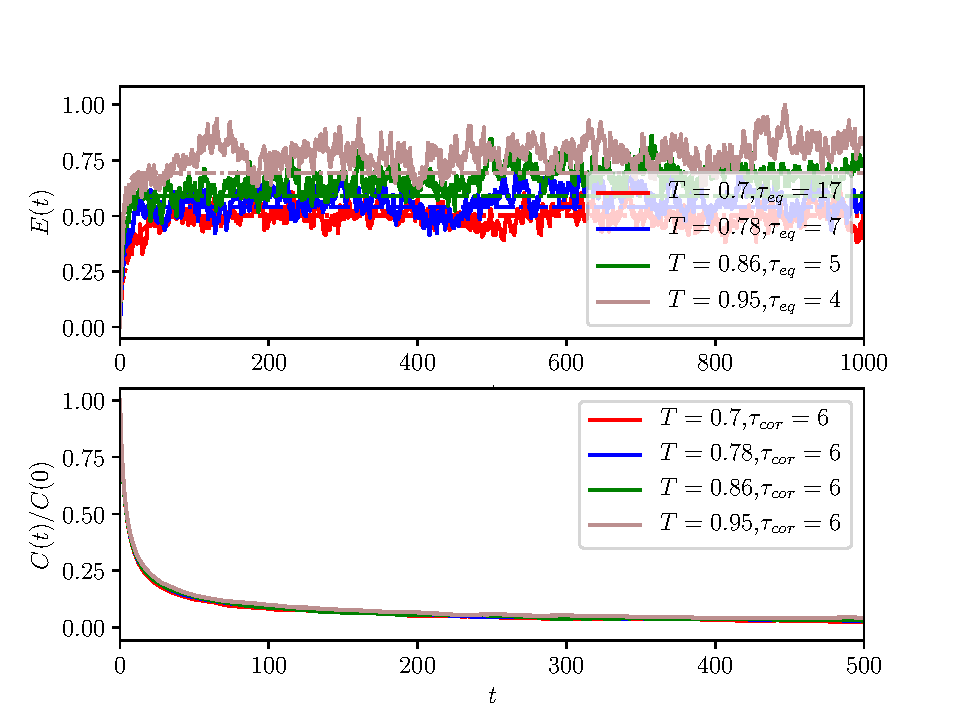
\includegraphics[scale=1]{numerical/sos-glau-eq-cor.pdf}
	\caption{Courbe de l'énergie (haut) et fonction d'auto-corrélation (bas) dansavec un algorithme de Glauber à partir d'une condition initiale à $T=\infty$, pour différentes températures.}
	\label{eq-glau}
\end{figure}

La différence d'énergie entre deux configurations est alors
\begin{align}
	\Delta E &= |h_{i-1}-(h_i + \alpha)| + |h_{i+1}-(h_i + \alpha)| - |h_{i-1}-h_i| - |h_{i+1}-h_i|  
\end{align}
Il n'est pas nécessaire de calculer la hauteur totale à chaque étape. La variable $\sum_i h_i$ peut être mise en mémoire, et mise à jour à chaque fois qu'une transition a été validée par la formule
\begin{align}
    <h>_{M+1} = <h>_M + \alpha
\end{align}
On peut faire de même pour la variable $\sum_i h_i^2$ , utile pour calculer la largeur de l'interface, ou bien l'énergie totale du système.

Afin d'accélérer le processus d'équilibrage du système, il est recommandé de commencer directement avec la valeur moyenne de magnétisation calculée à partir de la matrice de transfert. On regarde ensuite le temps d'équilibrage par la courbe $E(t)$, en attendant d'atteindre la valeur à l'équilibre. On choisit ici d'étudier l'énergie totale du système contrairement à la hauteur totale, puisqu'en absence de potentiel chimique, l'interface est libre de fluctuer entre $0$ et $L$. Dans la figure \ref{eq-glau}, on montre le temps d'équilibrage et le temps de corrélation du système en absence de potentiel chimique. Les temps assez faibles d'équilibrage te de corrélation assurent qu'une simulation équilibrée sur $10^3$ et mesurée sur $10^7$ étapes de Monte Carlo donneront des résultats précis.

Dans le modèle SOS, on s'attend à ce que les statistiques générées par la dynamique de Glauber soient identiques, comme on le voit dans la figure XXX.
{\color{red} rajouter figure où on voit $\sum_i h_i$ avec Glauber ET TM en fonciton de $\mu$ par exemple, pour prouver que ça marche.}
Dans ces conditions spéciales qui découlent de notre modèle, les simulations dans l'ensemble grand-canonique n'offrent que peu d'intérêt. Il n'existe cependant pas de matrice de transfert dans l'ensemble canonique, et c'est donc là que l'intérêt des simulations de Monte Carlo apparaît pour le modèle SOS.

%%%%%%%%%%%%%%
    \section{Algorithme de Kawasaki}
%%%%%%%%%%%%%%

Maintenant, on désire mettre au point un algorithme pour l'ensemble canonique, où la hauteur par site reste constante. Dans l'algorithme de Kawasaki \cite{kawasaki_diffusion_1966}, on choisit au hasard un site $i$ avec une probabilité $\frac{1}{L'}$, et un de ses deux voisins $i-1$ ou $i+1$ avec une probabilité $\frac{1}{2}$. Si par exemple on a choisit le site voisin $i-1$ (la discussion est la même pour le site $i+1$), on génère  la nouvelle configuration test d'Hamiltonien $H(h_0,...,h_{i-1}+1,h_i-1,...h_{L'})$. Ici, on a retiré une particule du site $i$ pour le transférer sur le site adjacent. 
La probabilité de sélection est à nouveau
\begin{align}
    g(C\to C') = \frac{1}{2L'}
\end{align}
et on choisit le même taux de transition  \ref{taux-transition-metropolis}.

Ici, on voit bien que la grandeur $\sum_i h_i$ est conservée au cours du temps. Dans le cas où le site $i$ donne une particule au site $i+1$, la différence d'énergie s'écrit	
\begin{align}
	\Delta E &= |h_{i-1}-(h_i - 1)| + |h_{i+1} + 1 -(h_i- 1)| + |h_{i+1} + 1-(h_{i+2} )|  \nn
	& - \left( |h_{i-1}-h_i| + |h_{i+1} -h_i| + |h_{i+1}-h_{i+2}| \right)
\end{align}

\begin{figure}[t]
	\centering
	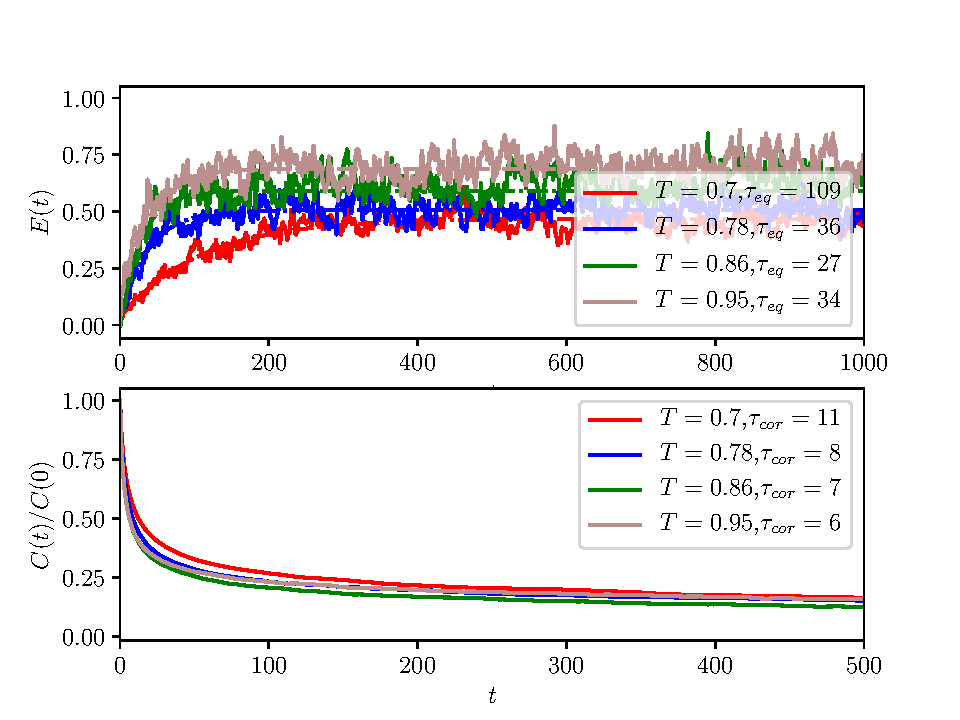
\includegraphics[scale=1]{numerical/sos-kaw-eq-cor.pdf}
	\caption{Courbe de l'énergie (haut) et fonction d'auto-corrélation (bas) avec un algorithme de Kawasaki à partir d'une condition initiale à $T=\infty$, pour différentes températures.}
	\label{eq-kaw}
\end{figure}
Dans la figure \ref{eq-kaw}, on remarque que le temps d'équilibrage et le temps de corrélation sont plus longs qu'avec la dynamique de Glauber. Bien que la dynamique soit plus lente parce que la longueur de corrélation dans le modèle A croît comme $t^\frac{1}{2}$ et comme $t^\frac{1}{3}$ dans le modèle B, on s'attend à ce que le temps de simulation reste similaire. 

Cette dynamique décrit la diffusion de particules au sein d'une interface. Il est donc possible de rajouter un flux qui brise l'équilibre. La méthode reste pertinente si on suppose que la dynamique du système reste lente comparée aux échanges de chaleur avec le réservoir. Dans ces conditions, on considère que les configurations $C$ respectent encore l'équilibre de Gibbs-Boltzmann. 

%%%%%%%%%%%%%%%%%%%		
    \section{Tips and tricks}
%%%%%%%%%%%%%%%%%%%    
    {\color{red} en annexe ou je peux le laisser dans le chapitre directement ? }
    La rapidité des simulations des modèles 1D soit rapide comparé aux modèles d'Ising est telle, qu'il est possible de simuler les phénomènes sur une plage plus grande de paramètres. Si une simulation de $10^/$ étapes de Monte Carlo dure en moyenne 20 minutes, le lancement d'une centaine de ces simulations peut vite prendre une journée ou plus.
    En C++, la première chose à faire pour gagner un facteur 5 dans le temps simulation est d'ajouter le flag d'optimisation $-03$ dans le compilateur, afin d'optimiser le code au niveau du préprocesseur. 
    
    Une fois cela fait, on se tourne vers le générateur de nombre pseudo-aléatoire (pRNG). En effet, à chaque étape de Monte Carlo on génère trois nombres aléatoires : 
    - le choix du site $i$
    - un booléen pour savoir si l'on rajoute ou enlève une particule dans le cas de la dynamique de Glauber,ou  un booléen pour savoir à quel plus proche voisin nous alons donner une particule dans le cas de la dynamique de Kawasaki
    - un double compris entre $[0,1]$ pour savoir si on accepte ou non la transition, dans le cas où $\Delta E \greater 0$
	La librairie C++ standard propose \textit{default\_random\_engine} comme générateur standard de nombres aléatoires. Un gain substantiel de temps d'un facteur 5 à 10 peut être fait en optant pour les générateurs \textit{sfc64} ou \textit{xoroshiro}. De plus, la génération d'un booléen ne requiert qu'un bit aléatoire, tandis que les générateurs classiques génères 64 bits à chaque fois, ce qui gâche 63 bits à chaque étape. Il est possible de mettre tous les bits générés en mémoire, afin de n'avoir à générer un nombre aléatoire qu'une fois tous les 64 booléens utilsés. Un exemple de code performant peut être trouvé ici
	 \url{https://martin.ankerl.com/2018/12/08/fast-random-bool/} 

    Pour finir, l'optimisation la plus évidente est la parallélisation du code. Bien que l'on puisse décomposer les domaines afin d'accélérer la simulation d'un système, les modèles 1D étant rapides, il est plus intéressant de procéder à une parallélisation basique sur les paramètres de la simulation (comme la température ou le potentiel chimique). En C++, il existe deux libraires : OpenMP et MPI. Il m'a fallu plusieurs pour comprendre que bien que la première soit très faicle d'implémentation, la parallélisation avec mémoire partagée rend le pRNG très instable, ce qui fausse complètement l'ensemble des simulations. Il est donc impératif d'utiliser la librairie MPI, qui assure l'étanchéité des pRNG entre chaque thread.
		
%%%%%%%%%%%%%%%%%%%%%%%%%%%%%%%%%%
\section{Conclusion}
%%%%%%%%%%%%%%%%%%%%%%%%%%%%%%%%%%

Dans ce chapitre, nous avons expliqué comment mesurer les moyennes statistiques des observables de nos systèmes grâce aux simulations de Monte Carlo Metropolis. 
Les hyopthèses sont les suivantes : on demande d'abord que le système soit à l'équilibre thermodynamique avec un réservoir de chaleur ; et on demande également que le système respecte le bilan détaillé. On obtient alors deux deux dynamiques possibles : la dynamique de Glauber permet de simuler les systèmes dans l'ensemble grand-canonique, tandis que la dynamique de Kawasaki permet de simuler les systpèmes dans l'ensemble canonique.
La première méthode est en parfait accord avec les reśultats de la matrice de transfert, et nous donne donc peu d'informations nouvelles.  C'est donc naturellement dans la dynamique de Kawasaki que les simulations de Monte Carlo pour un modèle SOS prennent tout leur sens.
On a également discuté du temps d'équilibrage et de corrélation, qui permettent d'obtenir des résultats précis en très peu de temps de calcul. Bien que ces simulations soient rapides comparé au modèle d'Ising (une vingtaine de minutes environ lorsque le code est optimisé), il est nécessaire d'optimiser le code via la parallélisation, ou un changement de pRNG.